\documentclass{beamer}

\usepackage[utf8]{inputenc}
\usepackage{adjustbox}
\usepackage[T2A]{fontenc}
\usepackage{amssymb}
\usepackage{amsmath}
\usepackage{mathrsfs}
\usepackage{euscript}
\usepackage{upgreek}
\usepackage[english,russian]{babel}
\usepackage{array}
\usepackage{theorem}
\usepackage[all]{xy}
\usepackage{subfig}
\usepackage{epstopdf}   
\usepackage{tikz}       
\usepackage{pgfplots}   
\usepackage{color}
\usepackage{ifthen}
\usepackage{url}
\usepackage{makeidx}
\usepackage{pb-diagram}
\usepackage{balance}
\usepackage{multirow} 
\usepackage{bibentry}
\usepackage{booktabs}
\usepackage{cmap}
\usepackage{amsthm}
\usepackage[linesnumbered,ruled,vlined]{algorithm2e}
\usepackage[absolute]{textpos}
\usepackage{fleqn,psfrag,wrapfig,tikz}
\usepackage{algpseudocode}
\usepackage{amsmath}

\usepackage{graphics}
\usepackage{graphicx} % Allows including images
\usepackage{tabularx}
%\usepackage{jmlda}
\usetheme{Warsaw}
\usecolortheme{sidebartab}
%\definecolor{beamer@blendedblue}{RGB}{15,80,120}
\DeclareMathOperator*{\argmax}{arg\,max}
%----------------------------------------------------------------------------------------------------------
\title[\hbox to 56mm{Нейросеть оптимальной сложности  \hfill\insertframenumber\,/\,\inserttotalframenumber}]
{Автоматическое построение нейросети оптимальной сложности}
\author[И.\,И.~Гридасов]{Илья Гридасов}
\institute{Московский физико-технический институт}
\date{\footnotesize{
\par\emph{Курс:} Численные методы обучения по прецедентам
(практика, В. В. Стрижов), группа 694, весна 2019
\par\emph{консультанты:} О.\,Ю.~Бахтеев, В. \,В.~Стрижов
\date{qq}
}}



\begin{document}

\begin{frame}
\titlepage % Print the title page as the first slide
\end{frame}

\begin{frame}
\frametitle{Построение нейросети оптимальной сложности}
\begin{block}{Цель исследования}
Предложить алгоритм поиска оптимальной архитектуры нейронной сети, найдя баланс между её сложностью и качеством. 
\end{block}
\begin{block}{Проблема}
Многие известные state-of-the-art нейросети требуют избыточно большого количества параметров, вследствие требуют большой выборки, поэтому часто не применимы на практике.
\end{block}
\begin{block}{Метод решения}
Ошибка декомпозируется на две независимые части - непосредственная ошибка алгоритма и стоимость описания его модели. Второй параметр оптимизиурется методом вариационного вывода.
\end{block}

\end{frame}

\begin{frame}
\frametitle{Существующие методы}

\textbf{Эволюционные методы}

\begin{itemize}
  \item Esteban Real, Alok Aggarwal, Yanping Huang, and Quoc V Le. Regularized evolution for image classifier architecture search, 2018.
  \item Hanxiao Liu, Karen Simonyan, Oriol Vinyals, Chrisantha Fernando, and Koray Kavukcuoglu. Hierarchical representations for efficient architecture search. ICLR, 2018b.
\end{itemize}

\textbf{RL методы}

\begin{itemize}
  \item Zhao Zhong, Junjie Yan, Wei Wu, Jing Shao, and Cheng-Lin Liu. Practical block-wise neural network
architecture generation, 2018.
  \item Hieu Pham, Melody Y Guan, Barret Zoph, Quoc V Le, and Jeff Dean. Efficient neural architecture
search via parameter sharing. ICML, 2018b.
\end{itemize}

\end{frame}

\begin{frame}
\frametitle{Постановка задачи поиска архитектуры}
\begin{block}{Дано}
Выборка размера m: $~ D_m = \{\textbf{x}_i, y_i\}_{i=1}^m,$

где $\textbf{x}_i \in \mathbb{R}^{n}$ - вектор признаков, $~y_i \in \mathbb{Y}$.

$\alpha$ - параметры архитектуры, $w$ - параметры модели.
\end{block}
\begin{block}{Функция ошибки}
Определим функцию ошибки на обучающей выборке $\mathcal{L}_{train}$ и на валидации $\mathcal{L}_{val}$, получаем задачу двух-уровневой оптимизации:
\begin{align}
	\min_\alpha \quad & \mathcal{L}_{val}(w^*(\alpha), \alpha) \label{eq:outer} \\
	\text{s.t.} \quad &w^*(\alpha) = \mathrm{argmin}_w \enskip \mathcal{L}_{train}(w, \alpha) \label{eq:inner}
\end{align}

\end{block}
\end{frame}

\begin{frame}
\frametitle{Постановка задачи поиска архитектуры}
\begin{block}{Декомпозиция ошибки}
Ошибку нейронной сети определим как минус логарифм правдоподобия $\mathcal{L}^N(w, \alpha, D) = -\ln Pr(D|w, \alpha) = -\sum \limits_{(x,y) \in D} \ln Pr(y|x, w, \alpha)$
\end{block}
\begin{block}{Вариационный вывод}
Зададим распределение на параметры $\mathcal{Q}(\beta)$, будем минимизировать вариационную свободную энергию: 
$$
\mathcal{F} = -\langle \ln \frac{Pr(D|w)P(w|\alpha)}{
\mathcal{Q}(w|\beta)} \rangle_{w \sim \mathcal{Q}(\beta)}
$$где $\langle \xi \rangle_{w \sim P}$ -  математичское ожидание величины $\xi$ по $w \sim P$. $\mathcal{F}$ раскладывается на две части:
$$
\mathcal{F} = \langle \mathcal{L}^N(w, D) \rangle_{w \sim \mathcal{Q}(\beta)}
+ D_{KL}(\mathcal{Q}(\beta)||P(\alpha))
$$
\end{block}
\end{frame}

\begin{frame}
\frametitle{Предлагаемый метод решения}

\begin{block}{Пространство поиска}
Представим архитектуру нейронной сети в виде графа вычислений, в котором каждая вершина зависит от предыдущих при помощи некоторой операций из фиксированного множества $\mathcal{O}$:
\begin{equation}
	x^{(j)} = \sum_{i<j} o^{(i, j)}(x^{(i)})
\end{equation}
\end{block}

\begin{block}{Непрерывная релаксация}
При помощи softmax можно сделать пространство поиска непрерывным.
\begin{align}
	\bar{o}^{(i,j)}(x) = \sum_{o \in \mathcal{O}} \frac{\exp(\alpha_o^{(i,j)})}{\sum_{o' \in \mathcal{O}} \exp(\alpha_{o'}^{(i,j)})} o(x)
	\label{eq:soft}
\end{align}

\end{block}

\end{frame}

\begin{frame}
\frametitle{Алгоритм оптимизации}

\begin{block}{Апроксимация градиента по \alpha}
Для эффективного поиска градиента по архитектуре воспользуемся следующей апроксимацией:
\begin{align}
&\nabla_\alpha \mathcal{L}_{val}(w^*(\alpha), \alpha) \\
\approx &\nabla_\alpha \mathcal{L}_{val}(w - \xi \nabla_{w} \mathcal{L}_{train}(w, \alpha), \alpha) \label{eq:single}
\end{align}
\end{block}

\begin{block}{Алгоритм}
\DontPrintSemicolon
Создать граф $\bar{o}^{(i,j)}$, параметризованный $\alpha^{(i,j)}$ для каждого ребра $(i,j)$ вычислительного графа\;

\While{веса меняются}{
	1. Обновить $\alpha$ шагом спуска
	$\nabla_\alpha \mathcal{L}_{val}(w - \xi \nabla_w \mathcal{L}_{train}(w, \alpha), \alpha)$\;
	\quad \;
	2. Обновить $w$ по градиенту $\nabla_w \mathcal{L}_{train}(w, \alpha)$\;
}
Вывести итоговую архитектуру по выученным весам \alpha.
\label{algo:pseudocode}
\end{block}

\end{frame}

\begin{frame}
\frametitle{Вычислительный эксперимент}
\begin{block}{Цель эксперимента}
Проверить работоспособность метода.
\end{block}

$\newline$

\textbf{Синтетическая выборка}

Выборка генерируется из распределения: 

$$
y_i \sim \alpha_0 \sin(w_0 x_i) + \alpha_1 \cos(w_1 x_i) + \mathcal{N}(0, 0.1)$$
$$ x_i \sim U[0, 1] $$
$w_0, w_1$ - выступают в качестве параметров модели, $\alpha_0, \alpha_1$ - параметры архитектуры.

\end{frame}

\begin{frame}
\frametitle{Результаты}
\begin{figure}[h!t]\center
Траектория спуска при разных значения параметра $\xi$ оптимизации.
\subfloat{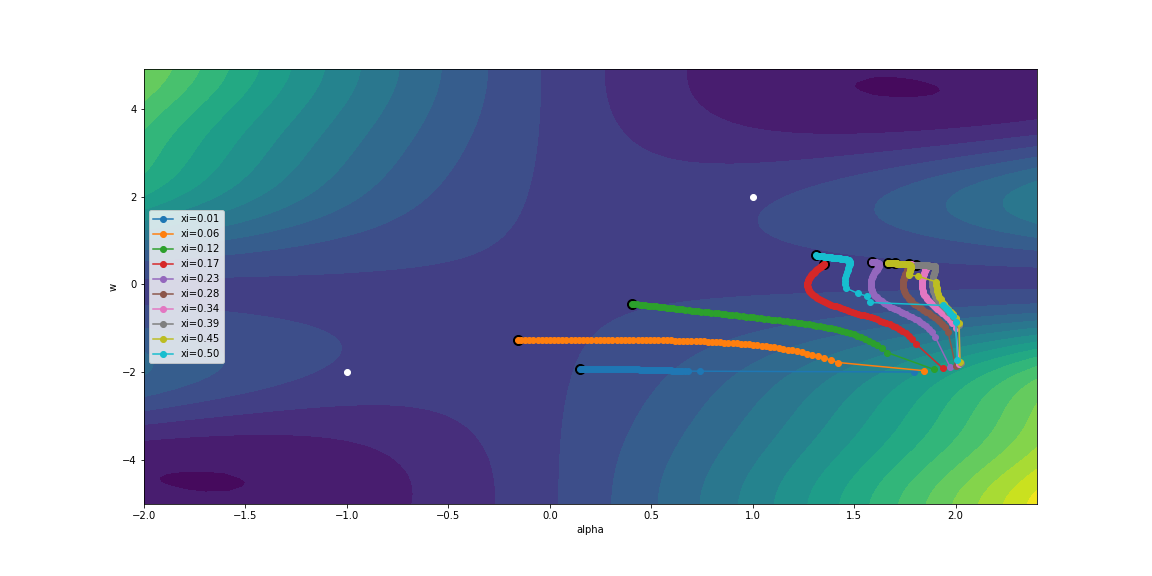
\includegraphics[width=1\textwidth]{surface_3.png}}\\

\caption{метод DARTS, синтетическая выборка}
\label{fig1}
\end{figure}
\end{frame}

\begin{frame}
\frametitle{Заключение}

\begin{itemize}
  \item Задача поиска оптимальной архитектуры сведена к задаче двух-уровневой оптимизации, для которой существуют эффективные приближенные методы.
  \item Показана работоспособность предложенного метода на синтетических данных.
  \item Далее предлагается применить данный метод на реальных данных, для оптимизации архитектуры глубоких нейронных сетей.
\end{itemize}

\end{frame}


\end{document}